\chapter{\IfLanguageName{dutch}{Stand van zaken}{State of the art}}
\label{ch:stand-van-zaken}

% Tip: Begin elk hoofdstuk met een paragraaf inleiding die beschrijft hoe
% dit hoofdstuk past binnen het geheel van de bachelorproef. Geef in het
% bijzonder aan wat de link is met het vorige en volgende hoofdstuk.

% Pas na deze inleidende paragraaf komt de eerste sectiehoofding.

% \texttt --> typewriter, bv. voor code
% \textcite --> de naam van de auteur in de text
% ~\autocite --> verwijzing achter de tekst


In dit hoofdstuk wordt uitgelegd wat Computer Vision en Computer Vision API’s zijn en inhouden. Tevens wordt een stand van zaken gegeven van het onderzoek naar beeldherkenning voor cultureel-erfgoedcollecties, de uitdagingen hierbij en experimenten met beeldherkenningstoepassingen in musea. 

\section{Computer vision}
\label{sec:cv}

%TODO glossariumtermen toevoegen
Computer Vision (CV) is het onderzoeksveld waarin technieken ontwikkeld worden om computers te helpen bij het zien en het begrijpen van de inhoud van digitale beelden zoals foto’s en video’s. Het is een deelgebied van Artifici\"{e}le Intelligentie en Machine Learning~\autocite{wikiCV}. Het doel van deze techniek is om computers te gebruiken voor taken met digitale beelden of video’s die normaal door mensen gedaan zouden worden. Computer Vision wordt momenteel met succes toegepast voor een breed scala van uitdagingen zoals inspectie van machines,  geautomatiseerde kassa-afrekeningen in de retail, motion capture, medische beeldvorming, bewaking en politieonderzoek, het herkennen van vingerafdrukken en het assisteren van mensen bij het identificeren van de inhoud van een foto of video~\autocite{Brownlee2019}.

De bovenvermelde uitdagingen gebruiken verschillende CV-taken voor het verkrijgen en analyseren van informatie uit de beelden, zoals beeldherkenning en bewegingsanalyse. Voor het onderzoek van deze bachelorproef is beeldherkenning de belangrijkste taak. Enkele typische voorbeelden hiervan zijn~\autocite{wikiCV}:
\begin{itemize}
	\item OCR: het identificeren van tekens in beelden van teksten;
	\item object classification: het classificeren van het beeld in een bepaalde categorie;
	\item object recognition: het identificeren van objecten in het beeld;
	\item object detection: het herkennen van een object of entiteit (zoals een persoon) en tevens aanduiden op het beeld waar het zich bevindt;
	\item face detection en recognition: het herkennen van personen en aanduiden waar ze zich op het beeld bevinden;
	\item content-based image retrieval: het vinden van beelden in een dataset met een bepaalde inhoud, bv. het vinden van gelijkaardige beelden.
\end{itemize}

%TODO meer referenties toevoegen in volgend puntje
% TODO glossarium
%TODO bekijk comments in google doc

Momenteel zijn algoritmes die gebaseerd zijn op Convolutional Neural Networks (CNN)\footnote{~Artificiële neurale netwerken zijn netwerken van verbonden neuronen die het mensenlijke brein nabootsen. Een CNN is een type neuraal netwerk waarbij niet alle neuronen met elkaar verbonden zijn en dat vooral toegepast wordt voor het analyseren van visuele beelden.} het best om deze taken uit te voeren. CNN voor beeldherkenning werd voor het eerst met succes geïntroduceerd in 2012. Sindsdien kent het veld van beeldherkenning een enorme groei. Artifici\"{e}le neurale netwerken, zoals CNN, leren taken uit te voeren op basis van een trainingsset. Als je wil dat het netwerk een bus herkent, dan bestaat de trainingsset uit verschillende voorbeelden van een bus, maar ook van wat een bus niet is. Wanneer, na de training, het model nieuwe beelden ziet, zou het moeten kunnen zeggen of het afgebeelde object een bus is of niet. Als het netwerk nog een andere taak moet uitvoeren, dan moet het netwerk nieuwe trainingsdata krijgen, bijvoorbeeld om te leren wat een fiets is~\autocite{Pokharna2016}. 

ImageNet is de dataset die meestal gebruikt wordt voor het ontwikkelen van toepassingen voor Computer Vision. ImageNet is een visuele databank die bestaat uit meer dan veertien miljoen beelden die annotaties hebben over wat er op de beelden staat. De databank voorziet 20.000 concepten, zoals ballon of aardbei. Elk van deze concepten bestaat uit enkele honderden beelden~\autocites{WikiImageNet}{Brownlee2019a}. Sinds 2010 vindt jaarlijks de ImageNet Large Scale Visual Recognition Challenge (ILSVRC) plaats. Hierbij wordt een beperkte set van ImageNet (één miljoen beelden voor duizend concepten) gebruikt om de performantie van de verschillende algoritmes te testen. Het valt hierbij op dat de resultaten jaarlijks enorm stijgen. Terwijl er in 2011 een foutenmarge was van 25\% voor de uitdaging van image classification, was dit tegen 2017 al teruggevallen tot 5\%. 

\textcite{Russakovsky2014} stellen vast dat domeinexperten beter blijven dan de CV-modellen, maar dat de CV-modellen significant beter scoren dan mensen die geen expert in het domein zijn. Mensen zijn bijvoorbeeld goed in het onderscheiden van een hond en een kat, maar een CV-model kan veel beter de verschillende hondenrassen herkennen. De modellen waren in het algemeen erg goed in het herkennen van verschillende soorten zoogdieren en hun rassen, maar hadden het veel moeilijker met metalen en doorzichtige voorwerpen. Ze hebben ook moeilijkheden met beelden die in meer dan vijf verschillende concepten te classificeren zijn\footnote{~De onderzoekers stelden vast dat ook menselijke classificatoren het hier moeilijk mee hadden.} en met het identificeren van kleine  objecten. Daarnaast hebben ze ook problemen met foto’s die vervormd zijn door het gebruik van kleurenfilters  of met abstracte voorstellingen van voorwerpen zoals 3D-rendered beelden, schilderijen, tekeningen en schetsen. Aangezien schilderijen, tekeningen, schetsen en objecten algemeen voorkomen in erfgoedcollecties, kan dit een probleem vormen.

\section{Computer Vision API}
\label{sec:CV-API}

%TODO glossarium
%TODO comments bekijken in google doc

CV API’s zijn REST API’s\footnote{API's zijn een set van commando's om met een webservice of computersysteem te communiceren.} die het developers mogelijk maken om machine learning toe te passen zonder hier zelf een expert in te zijn.  De services zijn zelf al getraind, waardoor het niet nodig is om zelf trainingsbeelden te voorzien en modellen te trainen. De meeste services bieden ook de mogelijkheid aan om eigen modellen te cre\"{e}ren. De diensten zijn zo toegankelijk dat iedere ontwikkelaar zonder machine learning expertise modellen kan bouwen. Volgens \textcite{Lardinois2018} zijn de services zo eenvoudig dat zelfs mensen zonder enige programmeerervaring de diensten kunnen gebruiken. De bekendste services zijn Clarifai\footnote{~\url{https://www.clarifai.com/}}, IBM Visual Recognition\footnote{~\url{https://www.ibm.com/watson/services/visual-recognition/}}, Microsoft Computer Vision\footnote{~\url{https://azure.microsoft.com/nl-nl/services/cognitive-services/computer-vision/}}, Amazon Rekognition\footnote{~\url{https://aws.amazon.com/rekognition/}} en Google Cloud Vision\footnote{~\url{https://cloud.google.com/vision/}}. 

Welke datasets gebruikt zijn om de CV API te trainen is niet duidelijk. Wel hebben zowel Clarifai, Google als Microsoft deelgenomen aan de ImageNet Challenge. In 2013 was ZFNet (Clarifai) de winnaar van de beeldclassificatietaak, in 2014 behaalde Google topresultaten voor objectdetectie met hun GoogLeNet-model en in 2015 behaalde Microsoft Research topresultaten met het ResNet-model. Op basis hiervan kunnen we veronderstellen dat de services minstens ImageNet gebruikt hebben~\autocite{Brownlee2019a}.

Het gebruik van de CV API’s is zeer toegankelijk. De meeste van deze CV API’s beschikken over een webinterface waarmee de service uitgetest kan worden en waarmee custom modellen gebouwd kunnen worden. Voor intensiever gebruik is er een REST API. Daarnaast hebben ze ook API clients\footnote{~API clients zijn implementaties van een API in een bepaalde programmeertaal.} in verschillende programmeertalen (o.a. Java, Python, Javascript/Node.js, C\#, PHP) die het de programmeur toelaat om de services te integreren in applicaties of scripts in een programmeertaal naar keuze. Beeldmateriaal kan op verschillende manieren aan de services bezorgd worden:
\begin{itemize}
	\item via een URL naar het beeld;
	\item in de vorm van base64;
	\item opgeslagen in het ecosysteem van de aanbieder (bv. S3 buckets voor Amazon Rekognition, of Google Cloud Storage buckets voor Google Cloud Vision).
\end{itemize}

De services kunnen verschillende aspecten van een beeld beschrijven:
\begin{itemize}
	\item OCR: het omzetten van tekens in beelden naar tekst;
	\item object detection: beschrijven van op het beeld aanwezige objecten of personen;
	\item algemene beschrijving van het soort beeld;
	\item de aard van het beeld (foto, tekening, schilderij)
	\item gezichtsherkenning: identificatie van bekende personen;
	\item landmarks: identificatie van bekende plaatsen;
	\item aboutness: emoties, sfeer en thema van het beeld;
	\item gebruikte kleuren, zowel hoofdkleuren als accentkleuren;
	\item NSFW-score: score op de aanwezigheid van content waaraan aanstoot genomen kan worden zoals erotiek, seksisme, racisme en geweld.
\end{itemize}

De resultaten worden meestal in de vorm van tags gegeven, maar ook taglines (een korte zin die het beeld beschrijft) of codes (kleurcodes) zijn mogelijk, net als URI’s (voor gelijkaardige beelden die op het web gevonden zijn). Bij de resultaten wordt steeds een waarschijnlijkheidsscore gegeven~\autocite{Vanstappen2019}.

Na een vergelijking van de top vijf van CV API’s was \textcite{Oberoi2016} onder de indruk van de resultaten. De services waren voldoende om informatie te krijgen over de kern van een beeld op een erg snelle en relatief goedkope manier.

\section{Computer vision voor cultureel erfgoed}
\label{sec:cv-voor-ce}

Er is al veel onderzoek gedaan naar het gebruik van Computer Vision voor cultureel-erfgoed. Omwille van de digitalisering blijven de beeldcollecties in musea en cultureel-erfgoedinstellingen groeien waardoor er een enorme registratie-achterstand is. Van CV wordt verwacht dat het het werk van de registratoren verlicht en de achterstanden wegwerkt. Computers worden hiervoor getraind als domeinexperten. Ze moeten van beelden van kunstwerken of erfgoedobjecten kunnen bepalen:
\begin{itemize}
	\item wie de kunstenaar of maker is;
	\item uit welk materiaal de werken gemaakt zijn; 
	\item in welke periode of jaar het werk gemaakt is;
	\item welk soort object het werk is;
	\item en tot welke kunststroming het werk behoort.  
\end{itemize}

%TODO glossarium

In zulke projecten trainen onderzoekers een eigen model of classifier om beelden van erfgoedobjecten te classificeren of te labelen. Een voorbeeld van zo’n onderzoek is het in 2017 gestarte Belgische INSIGHT-project waarin men wil onderzoeken of AI gebruikt kan worden voor het beschrijven voor museale collecties. De digitale collecties van de Koninklijke Musea voor Schone Kunsten van Belgi\"{e} en de Koninklijke Musea voor Kunst \& Geschiedenis worden als testcase gebruikt. Het einddoel van dit project is de ontwikkeling en release van een reeks praktische machine learning tools om digitale collecties te beheren~\autocite{UniAntwerpen2017?}.

\begin{figure}
	\centering
	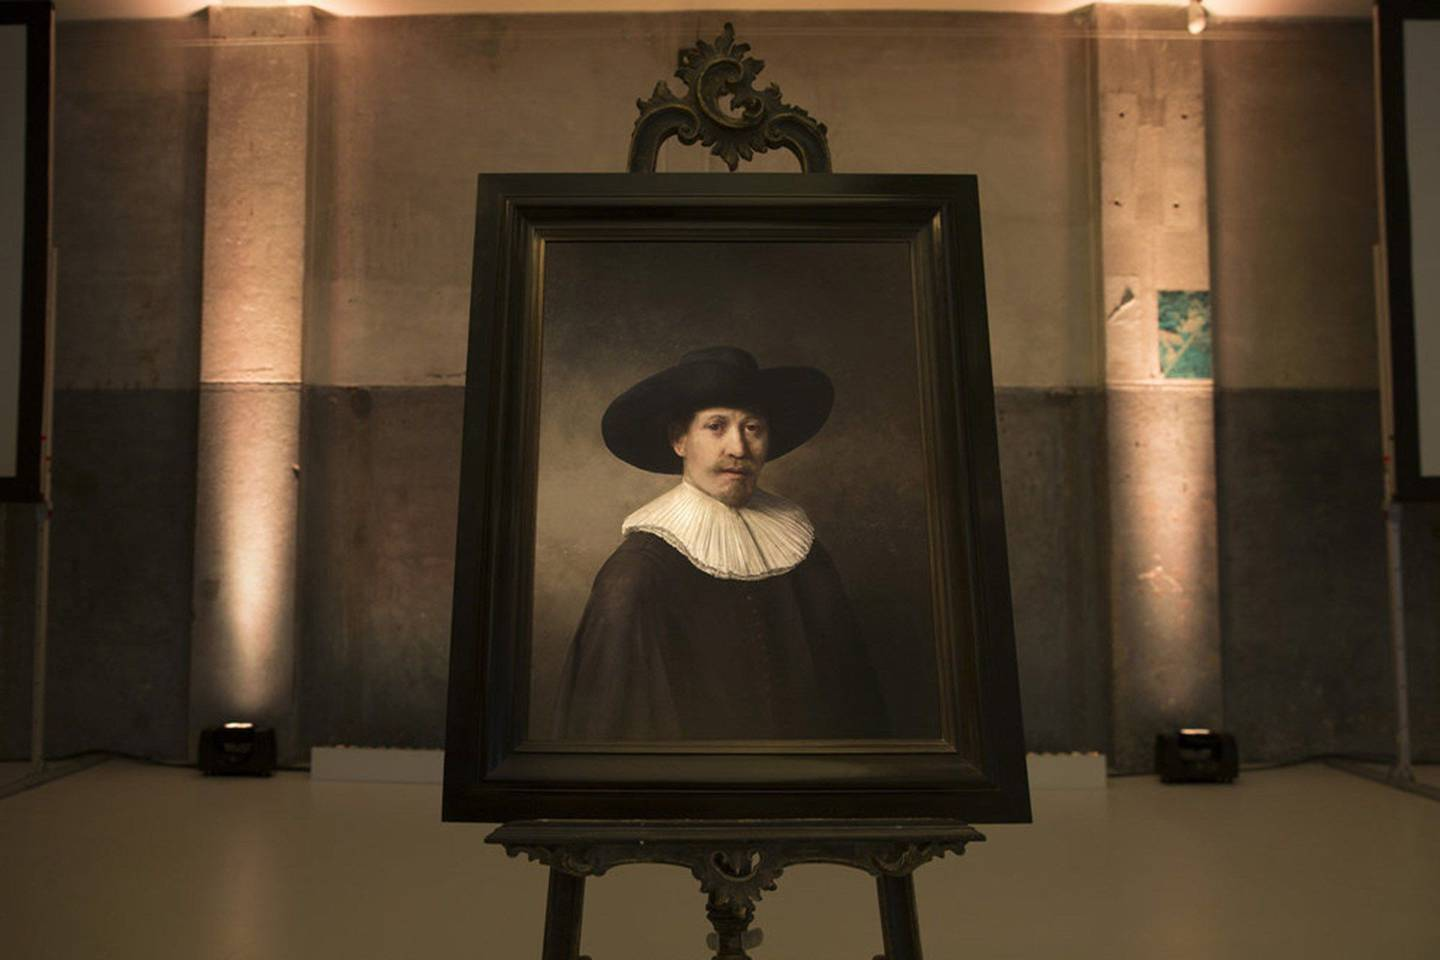
\includegraphics[width=\textwidth]{next-rembrandt.jpg}
	\caption[\textit{The Next Rembrandt}, een valse Rembrandt gecreëerd door een AI-algoritme]{\textit{The Next Rembrandt}, een valse Rembrandt gecreëerd door een AI-algoritme. Credit: Microsoft/ING/Delft University of Technology}
\end{figure}

Naast deze onderzoeken wordt ook onderzocht of CV gebruikt kan worden voor het herkennen van vervalsingen~\autocite{Dickson2018}, of om te verifi\"{e}ren of een kunstenaar een bepaald werk gemaakt heeft op basis van penseelstreken en potloodstrepen (ook om vervalsingen te ontdekken)~\autocite{Elgammal2017}. Daarnaast wordt AI gebruikt om nieuwe kunstwerken te maken\autocite{Dickson2019}. ING, Microsoft, TU Delft en Mauritshuis hebben in 2016 bijvoorbeeld zo een nieuw kunstwerk van Rembrandt gemaakt op basis van een databank van zijn schilderijen~\autocite{ING2016}.

\subsection{Uitdaging}
\label{subsec:cv-voor-ce-uitdaging}

Een probleem bij het gebruik van computer vision voor erfgoedobjecten zijn de veel kleinere datasets: 
%TODO  beetje inkorten
%TODO voetnoten en glossarium
\begin{itemize}
	\item \textcite{Blessings2013} cre\"{e}erden een dataset van 1.400 beelden via Google Images van de kunstenaars C\'{e}zanne, Dali, D\"{u}rer, Monet, Picasso, Rembrandt en Van Gogh (tweehonderd beelden per kunstenaar);
	\item \textcite{Mensink2014} ontwikkelden een dataset van meer dan 112.000 beelden van het Rijksmuseum die representatief is voor het museumcollectie. Het bestond uit 1.824 objecttypes waarvoor 406 verschillende soorten materialen gebruikt waren en overspande een periode van het het begin van onze jaartelling tot de late 19\textsuperscript{e} eeuw. De kunstwerken waren afkomstig van meer dan 6.000 kunstenaars. Het ging onder meer over schilderijen, foto’s, keramiek, en meubels.
	\item \textcite{Sabatteli2018} gebruikten die dataset van Mensink en Gemert, maar vulden dit aan met een kleinere dataset uit het DAMS Antwerpen.\footnote{Het DAMS Antwerpen is de online beeldbank van Musea en Erfgoed Antwerpen waarmee de collecties van de musea, bibliotheken, archieven en erfgoedinstellingen van de Stad Antwerpen in de kijker geplaatst wordt. Zie \url{https://dams.antwerpen.be}.} In totaal bestond de dataset uit ongeveer 100.000 beelden van kunstwerken die op te delen zijn in 2.016 materialen van kunstwerken, 135.809 beelden van kunstwerken die op te delen zijn in 1.677 objectsoorten en 90.674 beelden van kunstwerken van 2.099 kunstenaars.
	\item \textcite{Elgammal2018} gebruikten een dataset van 76.921 beelden van schilderijen afkomstig van 1.119 kunstenaars uit de 15\textsuperscript{e} eeuw tot de hedendaagse tijd.
\end{itemize}

Dit stelt weinig voor als je dit vergelijkt met de veertien miljoen beelden van ImageNet. Die beperking heeft te maken met copyright issues op beelden van kunstwerken en de afwezigheid van goede metadata bij de wel beschikbare beelden. 

Om dit probleem aan te pakken, verkenden zowel \textcite{Sabatteli2018} als \textcite{Elgammal2018} het veld van Transfer Learning. Hierbij worden geen neurale netwerken \textit{from scratch} gebouwd, maar worden reeds ontwikkelde netwerken verder gefinetuned. De onderzoekers gebruikten hiervoor neurale netwerken die \textit{state of the art} waren op de ImageNet Challenge. De artifici\"{e}le netwerken werd verder gefinetuned met de testdata. Beide onderzoeken toonden aan dat het beter was om de artificiële netwerken te finetunen dan zelf een model te bouwen~\autocite{Sabatteli2018}. \textcite{Elgammal2018} vermoedden dat betere resultaten mogelijk zijn met \textit{from scratch} netwerken als er grotere datasets ter grootte van ImageNet voor erfgoedobjecten ter beschikking zouden zijn.

\subsection{Resultaten}
\label{subsec:cv-voor-ce-resultaten}

Voor het classificeren van kunstwerken per kunstenaar behaalden \textcite{Blessings2013} goede resultaten (85\% correctheid). Hun onderzoek concentreerde zich wel maar op zeven kunstenaars. Bij de onderzoeken met meer kunstenaars, zoals bij van \textcite{Mensink2014} en \textcite{Sabatteli2018} waren de resultaten lager. Bij die laatste werd een maximumscore van 69\% behaald.

Het classificeren van werken per materiaal werd beschouwd als de eenvoudigste classificatie, onder meer omdat het aantal klassen vijf keer kleiner is dan bij de kunstenaarsclassificatie en typeclassificatie. \textcite{Sabatteli2018} vermoedden dat deze uitdaging ook het meest overeenstemt met de uitdagingen voor de ImageNet Challenge. Ze haalden hier een resultaat van 92,95\% op. \textcite{Mensink2014} behaalden een resultaat van 94\%. Ook voor het classificeren van kunstwerken per objecttype werden in beide onderzoeken gelijkaardige resultaten behaald.

Tot slot was ook het classificeren op basis van kunststroming succesvol. De uitdaging bestond uit het classificeren van 76.921 beelden in twintig kunststromingen. Er werd een score behaald van maximum 73\%. Ondanks dat het CV-model geen kennis heeft van kunstenaars, creatiedatum of geschiedenis van stijlen, worden de schilderijen uit dezelfde periode bij elkaar geplaatst en is er een geleidelijke overgang van stijlen te zien vanaf de Renaissance (15\textsuperscript{e} eeuw) tot de abstracte kunst (20\textsuperscript{e} eeuw)~\autocite{Elgammal2018}.

\newpage

\section{Experimenten met beeldherkenning in musea}
\label{sec:beeldherkenning-musea}

%TODO comments bekijken in google doc

Verschillende musea zijn reeds aan de slag gegaan met beeldherkenning via Computer Vision API’s. De use cases zijn anders dan bij het (academisch) onderzoek. Musea willen de bezoekers van hun website nieuwe ervaringen aanbieden om hun beeldcollectie te ontdekken, maar wensen tevens hun beelden beter doorzoekbaar te maken. Uit onderzoek blijkt namelijk dat gebruikers de behoefte hebben om beelden te kunnen zoeken op basis van inhoudelijke kenmerken, zoals identificeerbare objecten (\textit{Eiffeltoren}), generieke objecten (\textit{stoel}), iconologische thema’s (\textit{Het Laatste Avondmaal}) en abstracte begrippen (\textit{geluk})~\autocite{Vanstappen2019}. Om deze ervaringen aan te bieden, beginnen musea meer en meer te experimenteren met beeldherkenning.

The Museum of Modern Art (MoMA) gebruikt AI-diensten van Google om historische foto’s van afgelopen tentoonstellingen te koppelen aan de beelden uit de kunstcollectie die te zien zijn op die tentoonstellingszichten. Het CV-model analyseerde hiervoor alle foto’s van tentoonstellingen. Wanneer het model een kunstwerk op de foto herkende, dan legde het een koppeling met het beeld van het kunstwerk.~\autocite{MOMA2018?}. %TODO een afbeelding ofzoiets?

\begin{figure}
	\centering
	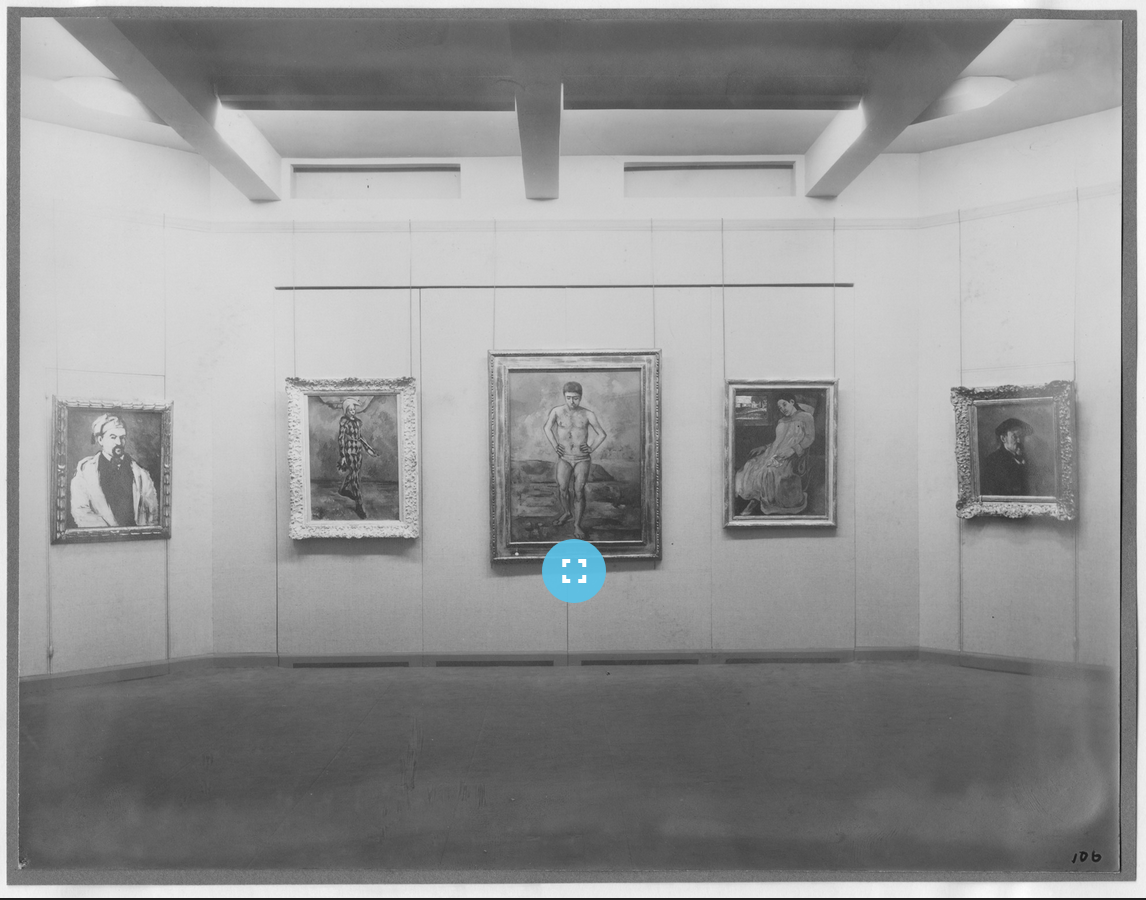
\includegraphics[width=0.620\textwidth]{MOMA_installatiezicht.png}\hfill
	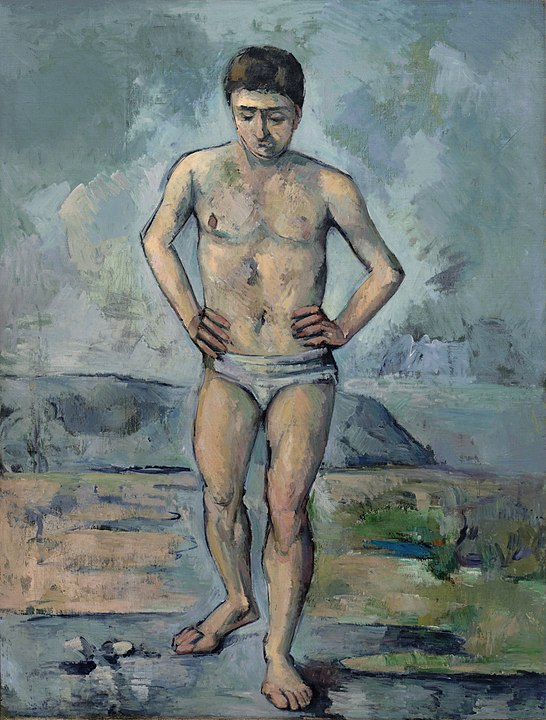
\includegraphics[width=0.370\textwidth]{MOMA_cezanne.jpg}\hfill
	\caption[Installatiezicht van MOMA waarin de AI-diensten van Google Arts \& Culture een schilderij van Cézanne herkennen]{In een installatiezicht van de tentoonstelling \textit{"Cézanne, Gauguin, Seurat, Van Gogh"} uit 1929 in het MOMA werd het werk \textit{De Bader} van Cézanne herkend (foto tentoonstelling: Photographic Archive. The Museum of Modern Art Archives, New York. IN1.7. Foto door Peter A. Juley.).}
\end{figure}

Voor het Noorse Nasjonalmuseet werd het deep learning framework Caffe\footnote{zie \url{http://caffe.berkeleyvision.org/}} gebruikt om compositionele gelijkenissen te zoeken tussen de kunstwerken en om ze te classificeren op basis van Iconclass\footnote{Iconclass is een classificatiesysteem voor kunst en iconografie, zie \url{http://www.iconclass.nl/home}}. Dit resulteerde in een vernieuwde publiekstoegang waarbij kunstwerken op basis van gelijkenissen gevisualiseerd werden. Hoe meer gelijkenissen een kunstwerk heeft, hoe dichter de kunstwerken bij elkaar staan~\autocite{Nasjonalmuseet2017?}. %TODO idem?

Daarnaast proberen een aantal musea via CV een oplossing te vinden voor de grote massa aan beelden die niet manueel beschreven raakt. Om zowel intern als extern gebruik van de beelden te stimuleren, zijn minstens een aantal trefwoorden nodig.
\begin{itemize}
	\item Wellcome Collection heeft zelf een model gemaakt en getraind om beelden te categoriseren en gelijkaardige beelden te clusteren. Het wordt intern gebruikt om ongewenste beelden te verwijderen van de collectiewebsite en om de registratieworkflow te verbeteren. In de toekomst wil men het mogelijk maken dat bezoekers van de collectiewebsite gelijkaardige beelden vinden op basis van een beeld~\autocite{Pim2018a}.
	\item Auckland Museum deed een test op tweeduizend collectiebeelden om via Microsoft Computer Vision de beelden automatisch te laten taggen en een basisrecord per beeld te creëren. Tags met een lagere waarschijnlijkheidsscore dan 60\% werden verwijderd om te vermijden dat beschamende of misleidende records gepubliceerd worden~\autocite{Moriarty2018a}.
	\item Het Britse webbedrijf CogApp gebruikte drie CV API’s (Clarifai, Google Cloud Vision en Microsoft Computer Vision) om een visuele zoekmachine te maken waarmee bezoekers op basis van de inhoudelijke kenmerken van de beelden doorheen een collectie kunnen zoeken.\footnote{Zie \url{http://labs.cogapp.com/iiif-ml/}.} Het deed de test met tweeduizend beelden van schilderijen van het Zweedse Nationalmuseum~\autocite{Hindle2017}.
	\item Sarjeant Gallery maakte zijn collectie op de nieuwe collectiewebsite doorzoekbaar via tags van een CV API.\footnote{Zie \url{https://collection.sarjeant.org.nz/explore}} De collectie kan doorzocht worden op basis van kleur, beeldoriëntatie en tags. De tags werden verkregen via de Google Cloud Vision. Foutieve tags worden verborgen door de collectiemedewerkers.~\autocite{Rowe2017} 
	\item Ook The Swedish National Heritage Board heeft een webinterface gecreëerd waarbij de collectie doorzoekbaar gemaakt wordt met onder meer tags van Google Cloud Vision~\autocite{Haskiya2019}.
\end{itemize} 

De resultaten met die experimenten waren goed. Soms zelfs beter dan verwacht. Sarjeant Gallery dacht de tags enkel te gebruiken voor intern gebruik. Collectiemedewerkers konden er sets van beelden rond een bepaald onderwerp mee maken. Men vond de tags echter zo goed dat besloten werd om ze ook op de website te publiceren. Doordat veel kunstwerken geen onderwerpbeschrijving hadden, konden de tags gebruikt worden om gerelateerde kunstwerken te vinden.~\autocite{Rowe2017}. Ook \textcite{Moriarty2018a} concludeert dat CV API nuttig zijn om snel basisrecords te creëren voor beelden waarmee zowel interne als externe gebruikers zich een weg kunnen zoeken doorheen de collectie. 

Er zijn wel nog vragen rond de controle op correctheid van de tags en hoe (en of) je aan de gebruiker moet laten weten dat de tags door een AI-systeem gecre\"{e}erd werden~\autocite{Moriarty2018a}. Volgens \textcite{Hindle2017} zijn foute beschrijvingen een gevolg zijn van het trainen van de CV API met hedendaagse beelden, terwijl erfgoedbeelden historisch zijn.

In Vlaanderen wordt eveneen ge\"{e}xperimenteerd met CV API. \textcite{Vanstappen2019} heeft voor MoMu onderzocht in welke mate off-the-shelf CV API zonder training bruikbaar zijn voor erfgoedcollecties. Het was een vergelijkend onderzoek waarbij verschillende modellen van Clarifai, Google Cloud Vision en Microsoft Computer Vision vergeleken werden op een set van 164 beelden van objecten (inclusief close-ups en detailfoto’s), catwalkbeelden, eventfoto’s en scenografie. \textcite{Vanstappen2019} concludeerde dat de verkregen tags voor een dergelijk gespecialiseerd onderwerp geen hoge kwaliteit hadden, maar dat ze wel bruikbare resultaten gaven voor een globale beschrijving van de erfgoedcollecties. Het sterke punt is vooral de performantie. Een API is veel sneller en goedkoper dan een menselijke registrator. Bovendien geeft de beeldherkenningssoftware ook onderwerpen die buiten de traditionele collectiebeschrijving vallen, zoals kleur en sfeer.

